\maketitle

Due: Wednesday, February 14 at 11:59 pm.

\section{Practice problems -- do not submit}
\subsection*{Chapter 10}
\begin{practice}p.802 \#63\end{practice}
\begin{pracsol}
  Observe that
  \[\begin{split}
    \|\br(t)\|^2 &= \cos^4(t)+\cos^2(t)\sin^2(t)+\sin^2(t) \\
    &= \cos^2(t)(\cos^2(t)+\sin^2(t))+\sin^2(t)\\
    &=\cos^2(t)+\sin^2(t)=1.
  \end{split}\]
\end{pracsol}
\begin{practice}p.812 \#13\end{practice}
\begin{pracsol}
  The position vector at time $t$ is $\br(t)=(t,t^2,t^2)$. The tangent vector at time $t$ is $\br'(t)=(1,2t,3t^2)$.

  The point $P=(1,1,1)$ corresponds to $t=1$, so the tangent vector at this point is
  \[\br'(1)=(1,2,3).\]
  Consequently, the tangent line to the curve at point $P$ is parametrized by the vector-valued function
  \[u\mapsto \br(1)+u\br'(1)=(1,1,1)+u(1,2,3).\]
  The parametric equations for the tangent line are
  \[x=1+u,\quad y=1+2u,\quad z=1+3u.\]
\end{pracsol}
\begin{practice}p.812 \#16\end{practice}
\begin{pracsol}
  The position vector at time $t$ is $\br(t)=(\ln(1+t),\frac1{1+t},-\frac1{(1-t)^2})$. The tangent vector at time $t$ is $\br'(t)=(\frac1{1+t},-\frac1{(1+t)^2},-\frac2{(1-t)^3})$.

  The point $P=(0,1,-1)$ corresponds to $t=0$, so the tangent vector at this point is
  \[\br'(0)=(1,-1,-2).\]
  Consequently, the tangent line to the curve at point $P$ is parametrized by the vector-valued function
  \[u\mapsto \br(0)+u\br'(0)=(0,1,-1)+u(1,-1,-2).\]
  The parametric equations for the tangent line are
  \[x=u,\quad y=1-u,\quad z=-1-2u.\]
\end{pracsol}
\begin{practice}p.823 \#9\end{practice}
\begin{pracsol}
  Since $\br'(t)=2t\cos(t^2)\bi+2t\sin(t^2)\bj+2t\bk$, $\|\br'(t)\|=\sqrt{8t^2}=2\sqrt2\,t,t\geq 0$. Therefore, the arc length calculation can proceed as follows.
  \[\int_0^{\sqrt\pi}\|\br'(t)\|\,dt=\int_0^{\sqrt\pi}2\sqrt2t\,dt=\sqrt2t^2\Big|_0^{\sqrt\pi}=\sqrt2\pi.\]
\end{pracsol}

\subsection*{11.1. Functions of several variables}
\begin{practice}p.872 \#11\end{practice}
\begin{pracsol}
  \[\begin{split}
    \left(h-\frac k3\right)\left(\frac12,3,0\right) &= h\left(\frac12,3,0\right)-\frac{k\left(\frac12,3,0\right)}{3}\\
    &= \frac12\cdot 9-\frac{\frac{3}{\frac12}}{3}=\frac52.
  \end{split}\]
\end{pracsol}
\begin{practice}p.872 \#12\end{practice}
\begin{pracsol}
  $\left(\frac hk\right)(3,4,-1)=xy^{z+1}(x+z)\Big|_{x=3,y=4,z=-1}=6$.
\end{pracsol}
\begin{practice}p.872 \#14\end{practice}
\begin{pracsol}
  $(\phi\circ g)(4,10)=\sqrt{x^2+2y}\Big|_{x=4,y=10}=\sqrt{4^2+2(10)}=6$.
\end{pracsol}
\begin{practice}p.872 \#15\end{practice}
\begin{pracsol}
  $(\phi\circ(2f+11g))(1,1)=\sqrt{2f(1,1)+11g(1,1)}=\sqrt{2\cdot\frac32+11\cdot 3}=6$.
\end{pracsol}
\begin{practice}p.872 \#45\end{practice}
\begin{pracsol}
  $f(f(x,y),f(x,y))=\frac{f(x,y)f(x,y)}{\sqrt{2f(x,y)^2}}$. This simplifies as follows.
  \[\begin{split}
    f(f(x,y),f(x,y)) = \frac{f(x,y)^2}{\sqrt2|f(x,y)|} &= \frac{\sqrt2}{2}|f(x,y)|\\
    &= \frac{\sqrt2}2\cdot\frac{|xy|}{\sqrt{x^2+y^2}}.
  \end{split}\]
\end{pracsol}

\newpage

\section{Homework problems -- submit these}

\begin{problem}
  An ant starts at $(0,0)$ and travels at a constant speed, in the shape of a square of side length 1, visiting the points $(1,0)$ at $t=1$, $(1,1)$ at $t=2$, $(0,1)$ at $t=3$, and back to $(0,0)$ at $t=4$.
  \begin{enumerate}[(a)]
    \item For each interval $0\leq t\leq 1,1\leq t\leq 2, 2\leq t\leq 3, 3\leq t\leq 4$, write down the vector-valued function $\br(t)$ that represents the ant's journey during that time interval.
    \begin{solution}
      For $0\leq t\leq 1$, $\br(t)=(t,0)$.

      For $1\leq t\leq 2$, $\br(t)=(1,t-1)$.

      For $2\leq t\leq 3$, $\br(t)=(3-t,1)$.

      For $3\leq t\leq 4$, $\br(t)=(0, 4-t)$.

      \textbf{Note}: Some students implicitly reset $t$ to 0 on each interval, getting different formulas. This is acceptable, but only if the resetting of $t$ to 0 was explicitly mentioned.
    \end{solution}
    \item We all know that the total length of the path that the ant traveled is the perimeter of the square, which is 4 units. But you're stranded on an island and must calculate it using the definition of arc length and evaluating the resulting integrals. Show that you get 4 units this way as well.
  \end{enumerate}
  \begin{solution}
    An impeccable solution by Marco Parete:

    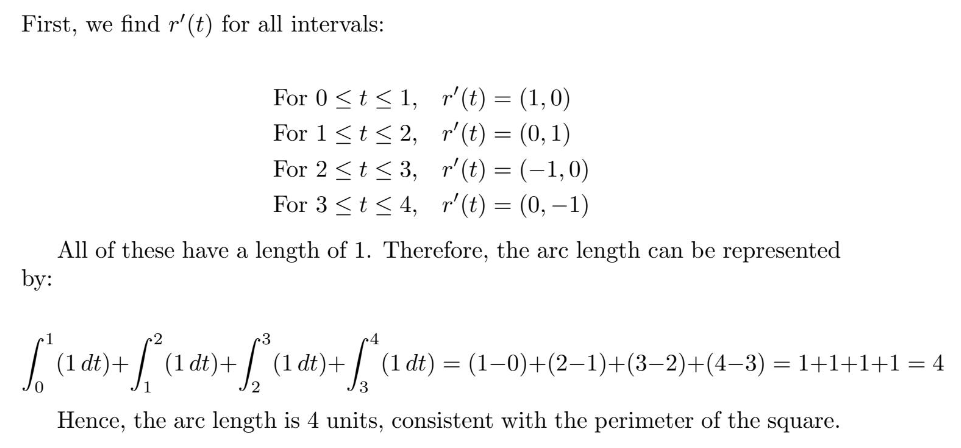
\includegraphics[width=\textwidth]{nice/p3.1b_marco.png}
  \end{solution}
\end{problem}

\begin{problem}\leavevmode
  \begin{enumerate}[(a)]
    \item Show that the curves $t\mapsto (t^3+t^2-3t+1,t^2,3t-1)$ and $t\mapsto(3t+1,2t,t^2+t-1)$ intersect at two points.
    \begin{solution}
      The system of equations to solve is:
      \begin{align*}
        t^3+t^2-3t+1 &= 3s+1\\
        t^2 &= 2s\\
        3t-1 &= s^2+s-1.
      \end{align*}
      Note that we need to use two independent variables because it is not necessarily the case that the points of intersection correspond to the same parameter $t$ for both curves. Indeed, the paths of two particles can cross while the particles themselves miss each other. (See p.774--775 for an example in the textbook about this.)

      We can take the second equation, rewrite it as $s=\frac{t^2}2$, and make that substitution into the first and third equation. Now we have two equations in $t$:
      \begin{align*}
        t^3+t^2-3t+1 &= \frac32t^2+1\\
        3t-1 &= \frac94t^4+\frac32t^2-1.
      \end{align*}
      Let's solve the first equation first, since is a polynomial equation of degree 3 while the other one has degree 4. This first equation simplifies to
      \[\begin{split}
        t^3-\frac12t^2-3t=0 &\iff t\left(t^2-\frac12t-3\right)=0\\
        &\iff t(2t^2-t-6)=0\\
        &\iff t(2t+3)(t-2)=0.
      \end{split}\]
      Therefore the first equation has solutions $t=0,-\frac32,2$. Out of these, the solutions $t=0$ and $t=2$ also satisfy the last equation $3t-1=\frac94t^4+\frac32t^2-1$.

      At $t=0$, the corresponding point is $(1,0,-1)$, and at $t=2$ the corresponding point is $(7,4,5)$. Thus, the two curves intersect at two points.

      \textbf{Remark}: This problem has the coincidence that the incorrect solution that uses 1 variable $t$ in both sides of the system of equations still gets the correct answer. This does not mean it is a valid solution, though.
    \end{solution}
    \item At each of these points, what is the angle between the tangent lines to the curves? (To clarify: at each point, what is the angle between the tangent line to the first curve at that point, and the tangent line to the second curve at the same point?)
    \begin{solution}
      Let $\br_1(t)$ and $\br_2(t)$ denote the lines $t\mapsto (t^3+t^2-3t+1,t^2,3t-1)$ and $t\mapsto(3t+1,2t,t^2+t-1)$ respectively. We have
      \begin{align*}
        \br_1'(0) &= (-3,0,3),& \br_2'(0) &= (3,2,1)\\
        \br_2'(2) &= (13,4,3),& \br_2'(2) &= (3,2,5).
      \end{align*}
      Therefore, if $\theta_1$ and $\theta_2$ denote the respective angles, we have
      \begin{align*}
        \cos\theta_1 &= \frac{(-3,0,3)\cdot(3,2,1)}{\|(-3,0,3)\|\|(3,2,1)\|}=\frac{-6}{6\sqrt7}=-\frac1{\sqrt7}\implies \theta_1=\cos^{-1}\left(-\frac1{\sqrt7}\right),\\
        \cos\theta_2 &= \frac{(13,4,3)\cdot(3,2,5)}{\|13,4,3\|\|(3,2,5)\|}=\frac{62}{\sqrt{7372}}\implies \theta_2=\cos^{-1}\left(\frac{62}{\sqrt{7372}}\right).
      \end{align*}
      Approximately we have $\theta_1\approx 1.96$ radians and $\theta_2\approx 0.764$ radians.
    \end{solution}
  \end{enumerate}
\end{problem}

\begin{problem}
  Usually when we divide two functions, as in $\frac{g(x,y)}{h(x,y)}$, where $h$ is non-constant, the resulting function will not be defined at some points. However, there are exceptions, where the resulting function is still defined for all $(x,y)\in\bR^2$. Find one such exception.
\end{problem}
\begin{solution}
  Some possibilities:
  \begin{itemize}
    \item $\frac{x+y}{x^2+y^2+1}$, defined everywhere because $x^2+y^2+1\neq 0$ for all $x,y\in\bR$.
    \item $\frac{xy^2}{e^x}$, defined everywhere because $e^x>0$ for all $x\in\bR$.
    \item $\frac{x-y}{\sin(x+y)+2}$, defined everywhere because $\sin(x+y)+2\geq -1+2=1>0$ for all $x,y\in\bR$.
  \end{itemize}
\end{solution}

\begin{problem}
  This example was briefly mentioned on the first day of this course. The functions
  \[f(x_1,x_2,\dots,x_{10000})=x_1x_2\cdots x_{10000}\]
  and
  \[g(x_1,x_2,\dots,x_{10000})=x_{10000}!\]
  are both functions in 10000 variables. Here, the notation $n!$ means the product of the positive integers from 1 to $n$ inclusive.
  \begin{enumerate}[(a)]
    \item Show that they are not the same function, by giving an input $(x_1,\dots,x_{10000})$ where they do not evaluate to the same value.
    \begin{solution}
      One possible input is $(x_1,\dots,x_{10000})=(2,1,\dots,1)$, since $f(2,1,\dots,1)=2\cdot 1\cdots 1=2$ while $g(2,1,\dots,1)=1!=1$.

      Another possibility is $(x_1,\dots,x_{10000})=(0,0,\dots,0)$, since $f(0,0,\dots,0)=0\cdots 0=0$ while $g(0,0,\dots,0)=0!=1$.

      Besides these, there are many other possible answers.
    \end{solution}
    \item Recall that factorial is defined only for non-negative integer inputs $0,1,2,\dots$. Given this information, what is the natural domain of $g$, in other words, the largest subset of $\bR^{10000}$ on which $g$ is defined?
    \begin{solution}
      $g(x_1,\dots,x_{10000})$ is defined as long as $x_{10000}$ is a non-negative integer. Therefore the domain of $g$ is $\{(x_1,\dots,x_{10000})\mid x_{10000}\geq 0\text{ and }x\text{ is an integer}\}$. There are plenty of equivalent correct formulations:
      \begin{itemize}
        \item $\{(x_1,\dots,x_{10000})\mid x_{10000}\text{ is a non-negative integer}\}$
        \item $\{(x_1,\dots,x_{10000})\mid x_{10000}\in\bZ\text{ and }x_{10000}\geq 0\}$
        \item $\{(x_1,\dots,x_{10000})\mid x_{10000}\in\bZ_{\geq 0}\}$
      \end{itemize}
      The following are common incorrect answers:
      \begin{itemize}
        \item $\{(x_1,\dots,x_{10000})\mid {\color{red}x_{10000}\geq 0}\}$ (missed the condition that $x_{10000}$ must be an integer)
        \item $\{(x_1,\dots,x_{10000})\mid {\color{red}\text{all }x_i\text{ are non-negative integers}}\}$ (missed that $x_1,\dots,x_{9999}$ is allowed take on non-integral values since $g$ is only taking the factorial of $x_{10000}$)
        \item {\color{red}$[0,\infty)$} (the main issue is that this describes a set of scalars, rather than a set of 10000-tuples (vectors with 10000 components). It also suffers from the above two issues)
      \end{itemize}

      7 out of 43 students answered this question completely correctly, so take care to read this solution 15 times. To assist in understanding, I will give more examples of functions and their domains below:
      \begin{itemize}
        \item The function $f(x)=x!$ has domain $\bZ_{\geq 0}$, the set of non-negative integers.
        \item The function $f(x,y)=y\cdot x!$ has domain $\{(x,y)\mid x\in\bZ_{\geq 0}\text{ and }y\in\bR\}$.
        \item The function $f(x,y,z)=(x^2)!$ has domain $\{(\pm\sqrt n,y,z)\mid n\in\bZ_{\geq 0}\text{ and }y,z\in\bR\}$. This can also be written as $\{(x,y,z)\mid y,z\in\bR\text{ and }x=\pm\sqrt n\text{ for some }n\in\bZ_{\geq 0}\}$.
        \item The function $f(x_1,x_2,\dots,x_{10000})=1/x_1$ has domain $\{(x_1,\dots,x_{10000})\mid x_1\neq 0\}$.
        \item The function $f(x,y)=\log(x-y)$ has domain $\{(x,y)\mid x>y\}$.
      \end{itemize}
    \end{solution}
    \item Find a tuple $(x_1,\dots,x_{10000})$ where the two functions are equal when evaluated at that input.
    \begin{solution}
      One example is $(x_1,\dots,x_{10000})=(1,2,\dots,10000)$. Then both $f(x_1,\dots,x_{10000})$ and $g(x_1,\dots,x_{10000})$ equal $10000!$.

      \textbf{Remark}: If you wrote something like ``$f=g$ when [...]'', avoid this in the future because the sentence $f=g$ means that the $f$ and $g$ are the same function, which means that they give the same output for \emph{all} possible inputs.

      \textbf{Remark}: A common mistake here is using $(1,2,3)$. While it is true that $1\cdot 2\cdot 3=3!$, the input $(1,2,3)$ is not a valid input for either $f$ or $g$, as $f$ and $g$ both require 10000 arguments in their input.
    \end{solution}
    \item The level set at $6$ for $g$ is the set $L_6=\{(x_1,x_2,\dots,x_{10000})\mid g(x_1,x_2,\dots,x_{10000})=6\}$. Describe this set. Why does it make sense to say that this set is 9999-dimensional?
    \begin{solution}
      We have
      \[\begin{split}
        L_6 &= \{(x_1,x_2,\dots,x_{10000})\mid g(x_1,x_2,\dots,x_{10000})=6\}\\
        &= \{(x_1,x_2,\dots,x_{10000})\mid x_{10000}! =6\}\\
        &= \{(x_1,x_2,\dots,x_{10000})\mid x_{10000} =3\}.
      \end{split}\]
      (Here we used the fact that $n!=6$ if and only if $n=3$.)

      This set is 9999-dimensional because there are 9999 free variables, namely $x_1,\dots,x_{9999}$, while the last variable $x_{10000}$ is fixed at 3. (This is the same way a plane like $x+y+z=3$ is 2-dimensional, because you can pick $x$ and $y$ to be anything, and for any choice you make, $z$ is uniquely determined.)
    \end{solution}
  \end{enumerate}
\end{problem}

\begin{problem}
  Let $f(x,y)$ be a function of 2 variables and let $\phi(t)$ be a scalar-valued function. Using $f$ and $\phi$ we can make a new function $g(x,y)=\phi(f(x,y))$. Let $c$ be a real number, let $L_c(f)$ denote the level set at $c$ for $f$, and let $L_{\phi(c)}(g)$ denote the level set at $\phi(c)$ for $g$. Prove that $L_c(f)$ is contained in $L_{\phi(c)}(g)$, by showing that every point in $L_c(f)$ is also in $L_{\phi(c)}(g)$.
\end{problem}
\begin{solution}
  Recall that $L_c(f)=\{(x,y)\mid f(x,y)=c\}$ and $L_{\phi(c)}(g)=\{(x,y)\mid g(x,y)=\phi(c)\}$.

  Let $(x,y)$ be a point in $L_c(f)$. We need to show that $(x,y)$ is also in $L_{\phi(c)}(g)$.

  $L_c(f)$ is the set of points $(x,y)$ satisfying $f(x,y)=c$. We have assumed that $(x,y)$ is in $L_c(f)$, so it follows that $f(x,y)=c$.

  This implies $g(x,y)=\phi(f(x,y))=\phi(c)$.

  This implies that $(x,y)$ is in $L_{\phi(c)}(g)$, which is what we wanted to prove.

  \textbf{Remark}: Making logical mathematical arguments is a skill many of you are still developing. Keep at it! It is recommended to read the above proof at least 15 times.

  \textbf{Remark}: The most common mistake is to invoke some sort of ``dividing both sides by $\phi$''. Remember that $\phi$ was a scalar-valued function, which is not the same as a scalar. You cannot cancel function applications as you would with scalar multiplication.
\end{solution}

\begin{problem}
  How difficult was each problem? Rate each problem (and part) on a difficulty scale from 1 to 7, where 1 means ``super easy, barely an inconvenience!'' and 7 means ``hardest problem I've ever done.''
\end{problem}

\newpage

\section{Hints}
\begin{hint}[Hint for 3]
  If you tried something like $\frac{(x-1)}{(x-1)}$, it doesn't work --- this is still undefined at $x=1$.
\end{hint}

\begin{hint}[Hint for 4(d)]
  If a variable does not appear in a formula for a function, changing its value does not affect the output of the function.
\end{hint}
